% ============================================================
%  Workshop Poster Set4MOST
% ============================================================

\documentclass[final]{beamer}

\usepackage[
  orientation=portrait,
  size=a0,
  scale=1.35
]{beamerposter}
 
\usepackage[utf8]{inputenc}
\usepackage[T1]{fontenc}
\usepackage[french]{babel}
\usepackage{graphicx}
\usepackage{amsmath}
\usepackage{xcolor}
\usepackage{tcolorbox}
\usepackage{booktabs}

% ── Colors ────────────────────────────────────────────────
\definecolor{Rouge}    {HTML}{C0272D}
\definecolor{RougeF}   {HTML}{8B0000}
\definecolor{GrisClair}{HTML}{F5F5F5}
\definecolor{Texte}    {HTML}{1A1A1A}

% ── Theme beamer ────────────────────────────────────────────
\usetheme{default}
\setbeamertemplate{navigation symbols}{}
\setbeamercolor{background canvas}{bg=white}
\setbeamercolor{block title}{fg=white,  bg=Rouge}
\setbeamercolor{block body} {fg=Texte,  bg=GrisClair}
\setbeamerfont{block title}{size=\large, series=\bfseries}
\setbeamerfont{block body} {size=\normalsize}

% ── Research Tracks Box ──────────────────────────────────────
\newcommand{\keybox}[1]{%
  \begin{tcolorbox}[
    colback=Rouge!10, colframe=Rouge,
    arc=3pt, boxrule=1.5pt,
    left=8pt, right=8pt, top=5pt, bottom=5pt
  ]
  \centering\large\bfseries #1
  \end{tcolorbox}}

% ============================================================
\begin{document}
\begin{frame}[t]{}

% ── Title head ────────────────────────────────────────────
\begin{columns}[c]

  \begin{column}{0.15\linewidth}
    \centering
    
\includegraphics[width=0.6\linewidth]{images/logoCEA.png}
  \end{column}

  \begin{column}{0.68\linewidth}
    \centering
    {\color{Rouge}\bfseries\Huge
	Navigation in unknown outdoor off-road envirronement using Interval Analysis}\\[0.6cm]
    {\large
      Celian \textsc{Daligault}$^1$$^2$,
      Eric \textsc{Lucet}$^1$,
      Sebastien \textsc{Lahaye}$^2$},
	  Sebastien \textsc{Lagrange}$^2$,
	  Remy \textsc{Guyonneau}$^2$\\[0.35cm]
    {\normalsize\color{gray}
      $^1$nano-innov, CEA — 2 Boulevard Thomas Gobert 91120 PALAISEAU France\quad
	  \newline
      $^2$LARIS, Universite Angers — 62 avenue Notre-Dame-du-Lac 49000 Angers France}\\[0.2cm]
    {\small\color{gray} celian.daligault@cea.fr}
  \end{column}

  \begin{column}{0.15\linewidth}
    \centering
    
\includegraphics[width=0.6\linewidth]{images/logoLARIS.png}
  \end{column}

\end{columns}

% ── Red separators heads ──────────────────────────────
\vspace{0.5cm}
\noindent\textcolor{Rouge}{\rule{\linewidth}{6pt}}\\[-2pt]
\noindent\textcolor{RougeF}{\rule{\linewidth}{2pt}}
\vspace{0.7cm}


\begin{columns}[T]

  % ── Left column (55 %) ───────────────────────────────
  \begin{column}{0.55\linewidth}

    \begin{block}{Context}
	Outdoor unknown off-road navigations stakes in mobile robotics application are multiples
	\newline
	In fact, Firstly, the unkown nature of the enviroonmeent necessitate to preform a full simulatuaous localisation and mapping (SLAM) whitout or with the least possible a priori hypothesis which is a well known and classical problem.
	\newline
	Then, the off-road specifity introduces many additional important information neccessary to know such as ground geometry, its nature (e.g. slipping ground) but also the presence and nature of dynamic objects to adjust the cartography models and potentially to avoid it when path generation is produced.
	\newline
	In addition, when a robot evolve outdoor, it face evolutionarry envirronement condition like a change in the luminosity and wheater conditions. This change in the envirronement does not always allow to use continusously the same sensors. A choice in the sensors but also multisensor fusion is consequently essential.
	\newline
	Moreover, the noisy nature of aquistion sensors must be a the subject of careful consideration to bring robust information from which path generation can be based on. The context of the described envirronement can easely correspond to applications such as construction or farming sites when vehicules evolve jointly with human operators, application when the security is the top priority. This last constraint justify how the use of the interval analysis should be considered.
	\newline
	Finally, a real application would necessitate real-time computation which means finding methods that are not too much costly in commputational load and memory.\\[0.5em]
    \end{block}

    \vspace{0.5cm}

	\begin{block}{A robust special sensor: The micro-wave radar}		
		What are the advantages or disadvantages ?\\[0.5em]
    \end{block}

    \vspace{0.5cm}

	\begin{block}{Overview of sensors integegration in the SLAM}

      \vspace{0.8em}
      \begin{center}
        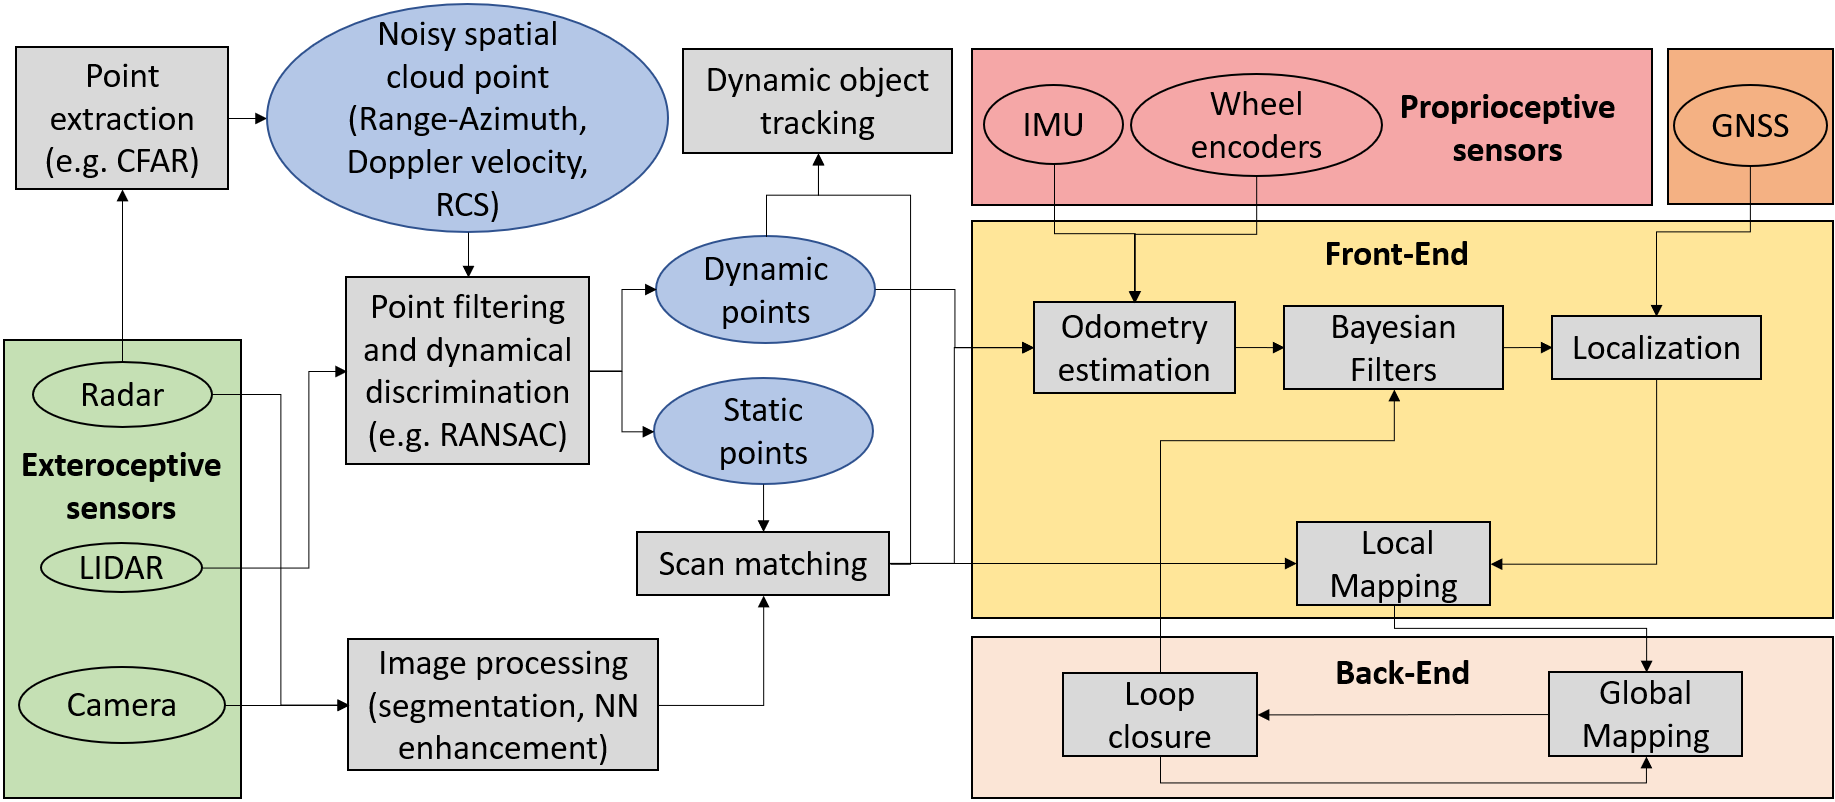
\includegraphics[width=0.92\linewidth]{images/Generalshema}\\[4pt]
        {\small\itshape Figure 1. Overview of the radar integration in SLAM.}
      \end{center}

    \end{block}


	\begin{block}{Dynamic object in the envirronement}		
		There is a two main kind of obstacles: semi-static and highly dynamic.\\[0.5em]
    \end{block}

	\begin{block}{The visibility problem}
      {
		One of the main issue of shape free hypothesis is that only face is 
      }
    \end{block}

  \end{column}


  % ── right column (35 %) ───────────────────────────────
  \begin{column}{0.35\linewidth}

	\begin{block}{An application of the radar benefit: The dynamic tracking}
      {
		Classically, when range-azimuth sensors are used, dynamic object tracking is performed by comparaison of multiple frame to be able to detect dynamicity. 
		\newline
		The additional measure of Doppler Velocity allow (that is generally included in radar output) for instantanuous motion information. In fact, the radial velocity when is combined with spatial points allow to refine the velocity estimation model but also to retrieve the rotational velocity and therefore, measure rotation
      }
    \end{block}

	\vspace{0.5cm}

	\begin{center}
		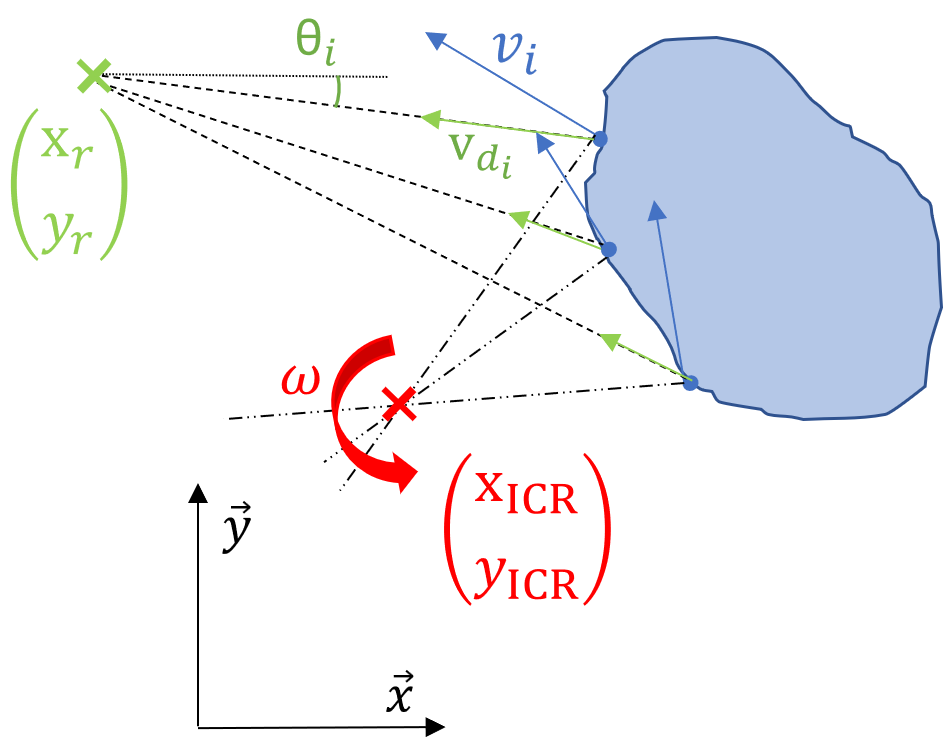
\includegraphics[width=0.92\linewidth]{images/ICRretrieval.png}\\[4pt]
		{\small\itshape Figure 1. ICR and angular velocity retrieval with distribution of radial velocity.}
	\end{center}

	\vspace{0.5cm}

    % Research Tracks
    \begin{tcolorbox}[
      title={\large\bfseries\color{white} Research tracks},
      colbacktitle=Rouge,
      colback=Rouge!12,
      colframe=Rouge,
      arc=3pt, boxrule=1pt,
      left=8pt, right=8pt, top=6pt, bottom=6pt
    ]
      Réponse directe à la question de recherche.\\[0.4em]
      Implication principale (clinique ou théorique).\\[0.4em]
      Perspective à court terme.
    \end{tcolorbox}

    \vspace{0.5cm}

    \begin{block}{Bibliography}
      {\footnotesize
      [1] Auteur et al. \textit{Journal}. Année;Vol:Pages.\\[3pt]
      [2] Auteur et al. \textit{Journal}. Année;Vol:Pages.\\[3pt]
      [3] Auteur et al. \textit{Journal}. Année;Vol:Pages.
      }
    \end{block}

    \vspace{0.5cm}

  \end{column}

\end{columns}

% ── Low Red  ──────────────────────────────────────
\vspace{0.7cm}
\noindent\textcolor{RougeF}{\rule{\linewidth}{2pt}}\\[-2pt]
\noindent\textcolor{Rouge}{\rule{\linewidth}{6pt}}

\end{frame}
\end{document}